\documentclass[11pt, a4paper]{jarticle}
% \documentclass{jarticle}

%% 【%】を用いた以降のその行の分を無視する
%% よって【%】はコメントアウトに使用できる

% \input{sonota/aislab_discuss} %% ディスカッション資料用の設定を読み込む
\usepackage{style/aislab}

\pagestyle{empty} %% ページ番号を消す

%% 図の挿入可
\usepackage[dvipdfmx]{graphicx} %% ←たぶんこれが一番楽
\usepackage[]{style/lastpage}
\usepackage{subcaption}

\usepackage[backend=bibtex,sorting=none]{biblatex}
\addbibresource{references.bib}
\defbibheading{bibliography}{\section*{参考文献}}

%%%%%%%%%%%% ページを分数形式
\makeatletter
\def\ps@myplain{\let\@mkboth\@gobbletwo%
\let\ps@jpl@in\ps@plain
\let\@oddhead\@empty
\def\@oddfoot{\reset@font\hfil- \thepage / \pageref{LastPage} -\hfil}% lastpage.tds.zipを使うことで x/最終ページ でページ数を表示できる
\let\@evenhead\@empty
\let\@evenfoot\@oddfoot}
\makeatother
\pagestyle{myplain}

% 図はfigsのサブディレクトリに集めることにする.
\graphicspath{{./figures/}}

\renewcommand{\figurename}{Fig.}
\renewcommand{\tablename}{Table}

%%%%%%%%%%%%%%%%%%%%%%%%%%%%%%%%%%%%%%%%%%%%%%%%%% ▽本文開始▽
\begin{document}


%% タイトルの設定
\jptitle{第0回:春の講習会(Docker + LaTeX)} %% 日本語タイトル
\entitle{0th :Spring Seminars(Docker + LaTeX)} %% 英語タイトル
\author{B3 塚 春輝} %% 氏名
\date{2025/03/11} %% 日付

\maketitle %% タイトル作成



%%%%%%%%%%%%%%%%%%%%%%%%%%%%%%%%%%%%%%%%%%%%%%%%%%%%%%%%%%%



%%%%%%%%%%%%%%%%%%%%%%%%%%%%%%%%%%%%%%%%%%%%%%%%%%%%%%%%%%%
\section{AISLab の概要}
Advanced Intelligent System Laboratory (以降;AIS Lab.) は,立命館大学情報理工学部実世界情報
コースの研究室である.2024年度時点の指導教員は,李 周浩教授,Tran Dinh Tuan助教,藤井 康之
特任助教の3人である.また,多くの学生が在籍し,2024年度の秋学期には40人の学生が在籍している.
2024 年度秋学期の学年別在籍人数を Table 1 に示す.

\section{知能化空間と MoMo}
本研究室で行われてきた研究テーマの一つとして,知能化空間(Intelligent Space:以降,iSpace)\cite{dd}
がある.iSpaceとは,センサネットワークに基づいた拡張環境システムであり,ユーザに様々なサービス
を提供可能な空間である.Fig.1は,iSpaceの概要を表す図である.iSpaceでは,分散知能ネットワーク
デバイス(Distributed Intelligent Network Devices:以降,DIND)が壁や天井に設置されている.ユー
ザの要求と空間的状況は,カメラやマイクなどのDINDのセンサによって認識され,iSpaceのすべての
DIND に共有される.プロジェクタ,スピーカやロボットなどの出力デバイスを備えたDINDは,認識さ
れた結果に基づいて適切なサービスを行う.これによって空間内のユーザに対する情報的・物理的なサー
ビスの提供を実現できる.この研究分野に対しては,多様なアプローチの研究が行われている.

しかし,様々な空間の状況を把握し,適切なサービスを行うためには,多数のデバイスが空間に配置
されたり,各サービスに合わせてデバイスの位置が適宜変更されたりする必要がある.これらはコスト
がかかり,固定されたデバイスを逐一手作業で再配置するのは現実的ではない.この問題に対して,移
動ロボットによる空間内のデバイスの再配置を行う再構成可能な知能化空間(ReconfigurableIntelligent
 Space:以降,R+iSpace)の提案がされた\cite{ee}.R+iSpace では,DIND を含む様々なデバイスを搭載し
て壁面または天井面を自由に移動するロボットとして,MobileModule(以降,MoMo)が開発された.

\section{本日の内容}
本章では,本日の講習会の内容を簡単に説明する.
\subsection{GNU/Linux コマンド}
GNU/Linux コマンドは,CLI で Linux を操作するためのコマンドである.”ls” コマンドは,〇〇を
行い,”cat” コマンドは,〇〇を行う.
\begin{table}[b] %% h=この場所,t=ページ上,b=ページ下,p=単独ページ  %% t>b の順で図の挿入場所が優先される
	\caption{2024年度秋学期の学年別在籍人数}
	\label{table1}
	\begin{center}
	\begin{tabular}{ c || c}
	\hline
	学年 & 在籍人数[人] \\ \hline
	\hline
	D3 & 1  \\ 
    D2 & 2  \\ 
    D1 & 1  \\ 
    M2 & 6  \\ 
    M1 & 8  \\ 
    B4 & 10  \\ 
    B3 & 12  \\ \hline
    合計 & 40  \\ \hline
	\end{tabular}
	\end{center}
\end{table}

\begin{figure}[tb] %% h=この場所,t=ページ上,b=ページ下,p=単独ページ  %% t>b の順で図の挿入場所が優先される
	\begin{center}
	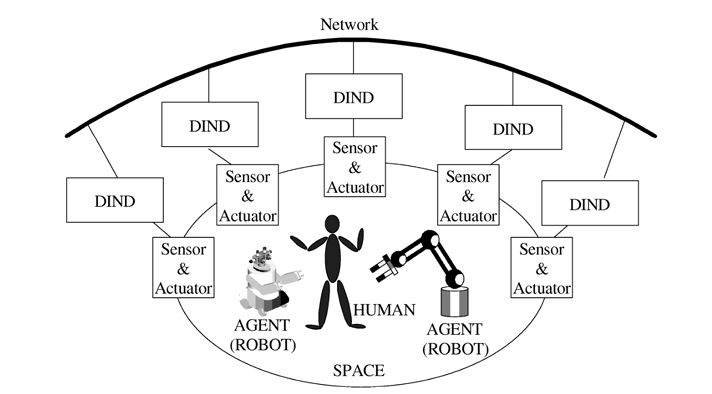
\includegraphics[width=\linewidth]{figure3.png}
	\caption{Outline of iSpace[1]}
	\label{figure1}
	\end{center}
\end{figure}

\begin{figure}[tb]
    \centering
    \begin{minipage}{0.45\textwidth}
        \centering
        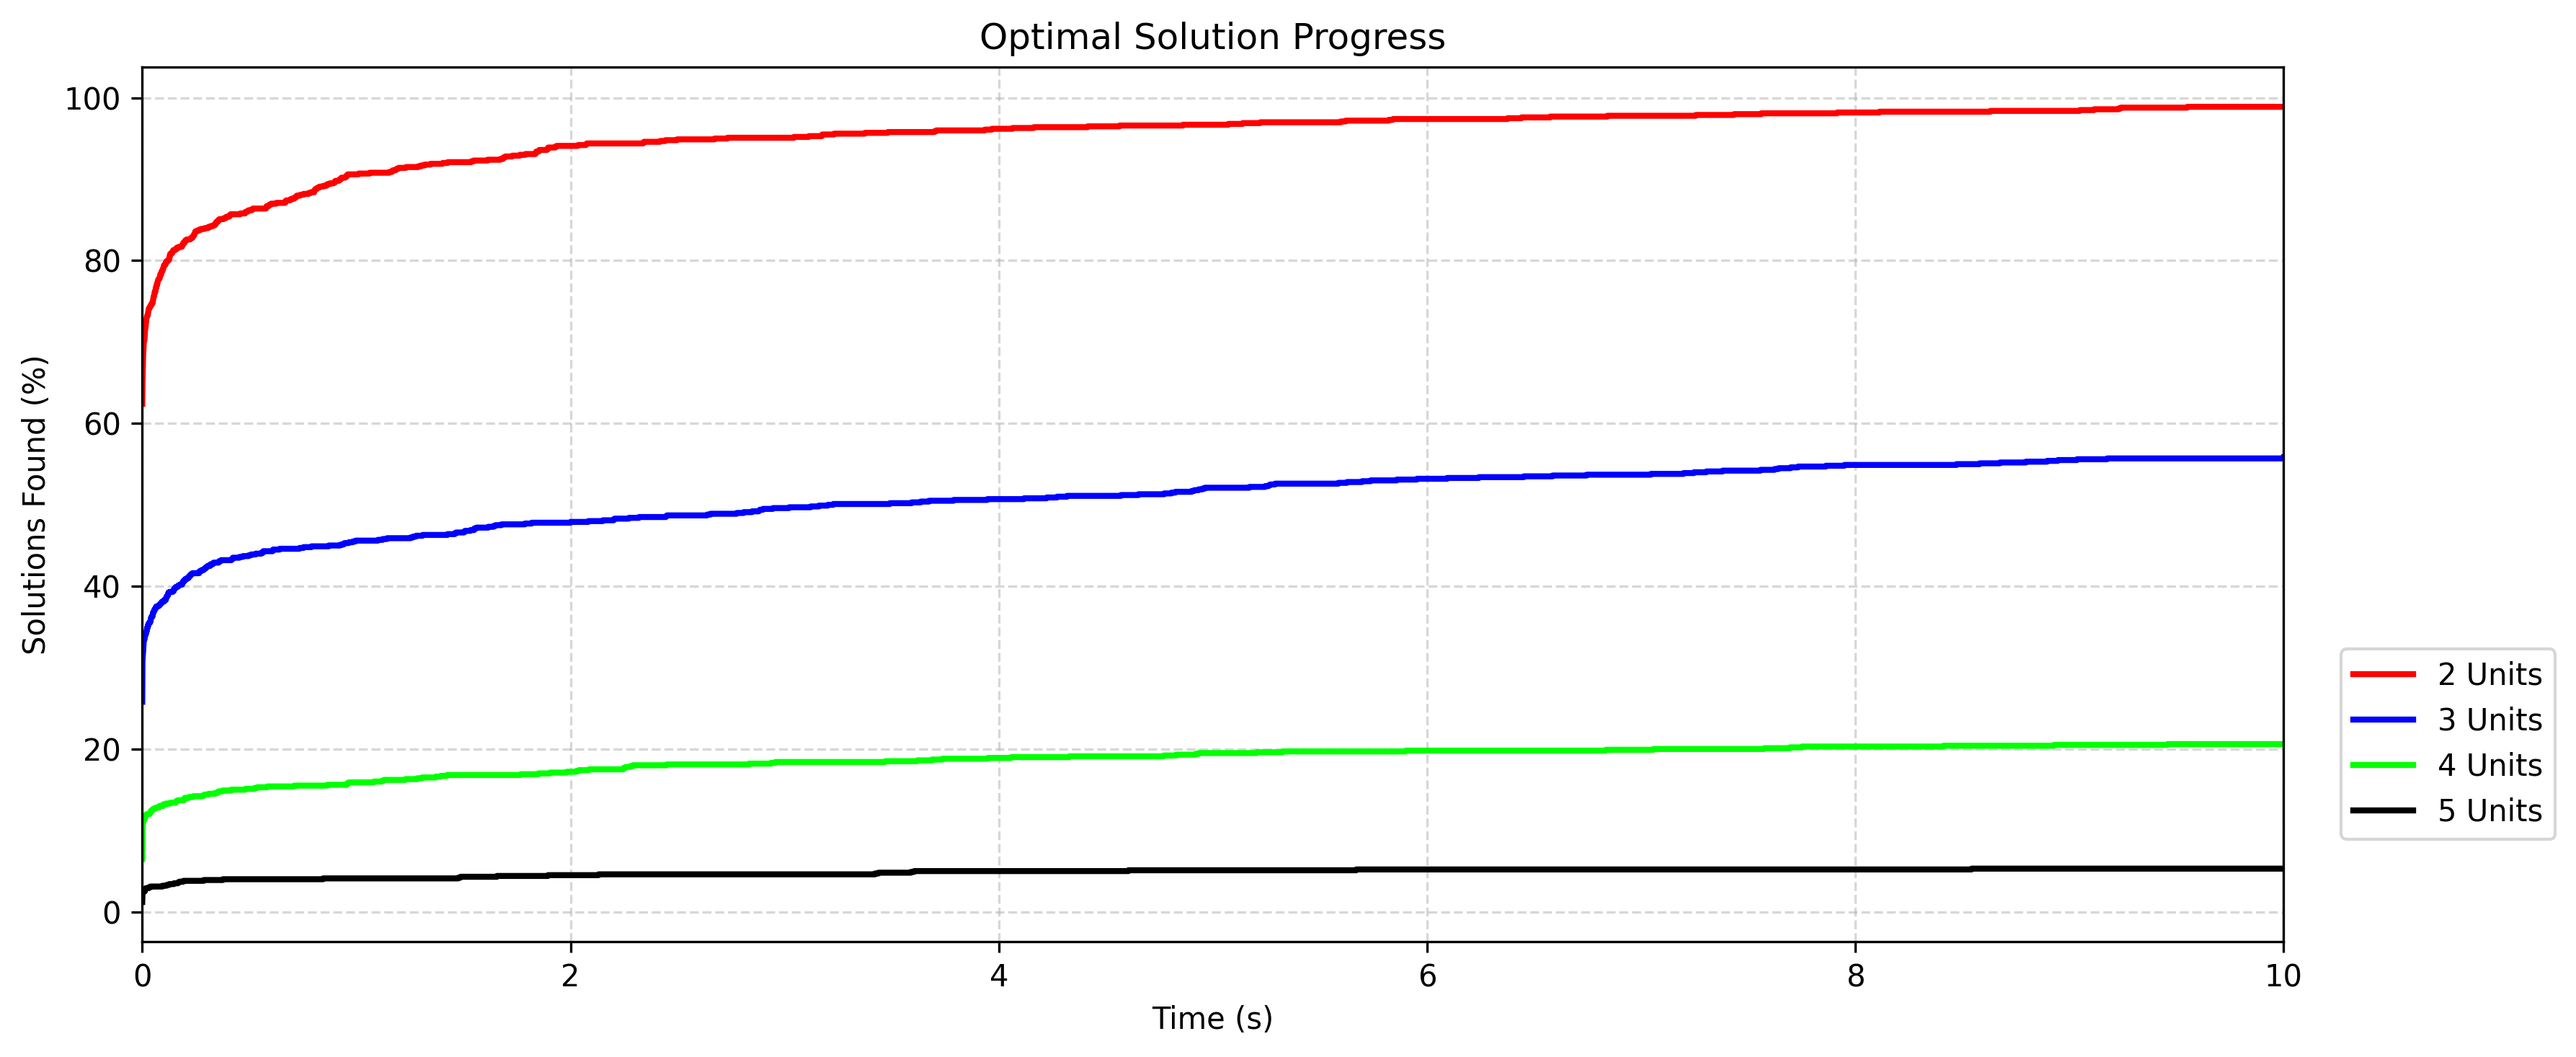
\includegraphics[width=\linewidth]{solution_progress_final.png}
		\subcaption{Graph 1}
    \end{minipage}
    \hfill
    \begin{minipage}{0.45\textwidth}
        \centering
        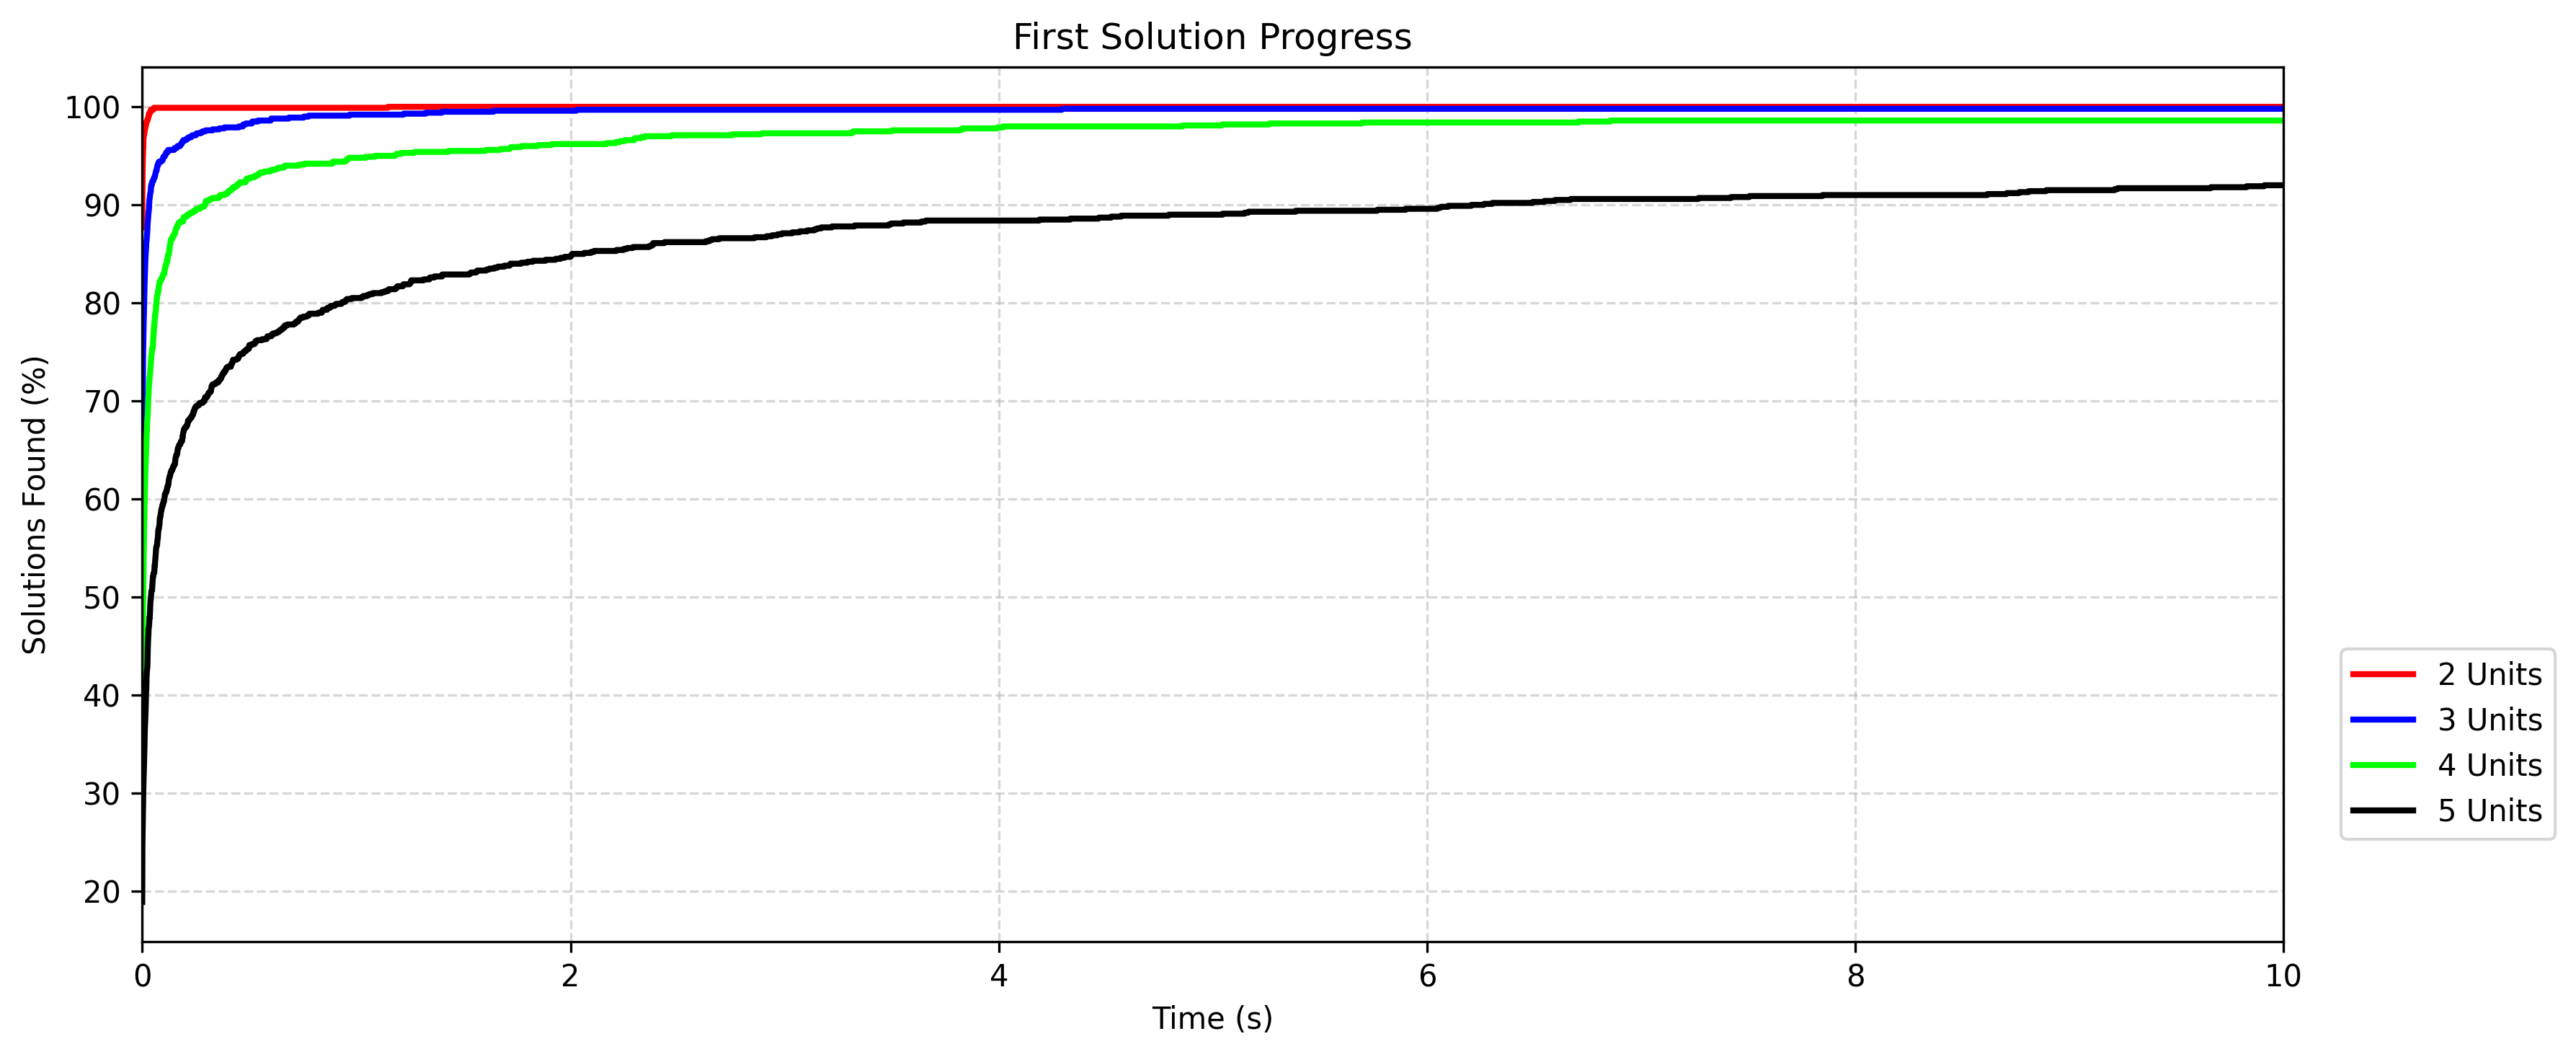
\includegraphics[width=\linewidth]{solution_progress_first.png}
		\subcaption{Graph 2}
    \end{minipage}
    \caption{Output image}
\end{figure}

\subsection{Docker}
Docker は,コンテナ型の仮想化ソフトウェアの一種である.Dockerコンテナは,〇〇を実行すること
によって作成される.また,〇〇とよばれるソースコードによって,任意のコンテナ構成を作成すること
ができる.本講習で作成したコンテナでサンプルプログラムを実行して得られた画像をFig.2に示す.

\subsection{LaTeX}
LaTex は文書作成のためのソフトウェアであり,主にアカデミアにおいて論文執筆などに用いられる.

\section{質問・感想}
自由に書いてください.(任意)

\printbibliography

\end{document}